\documentclass[tikz,border=-20pt]{standalone}
\tikzstyle{arrow} = [thick,->,>=stealth]
\usetikzlibrary{external}
\tikzexternalize
\begin{document}
\begin{tikzpicture}
    \node[anchor=south west,inner sep=0] (image) at (0,0) {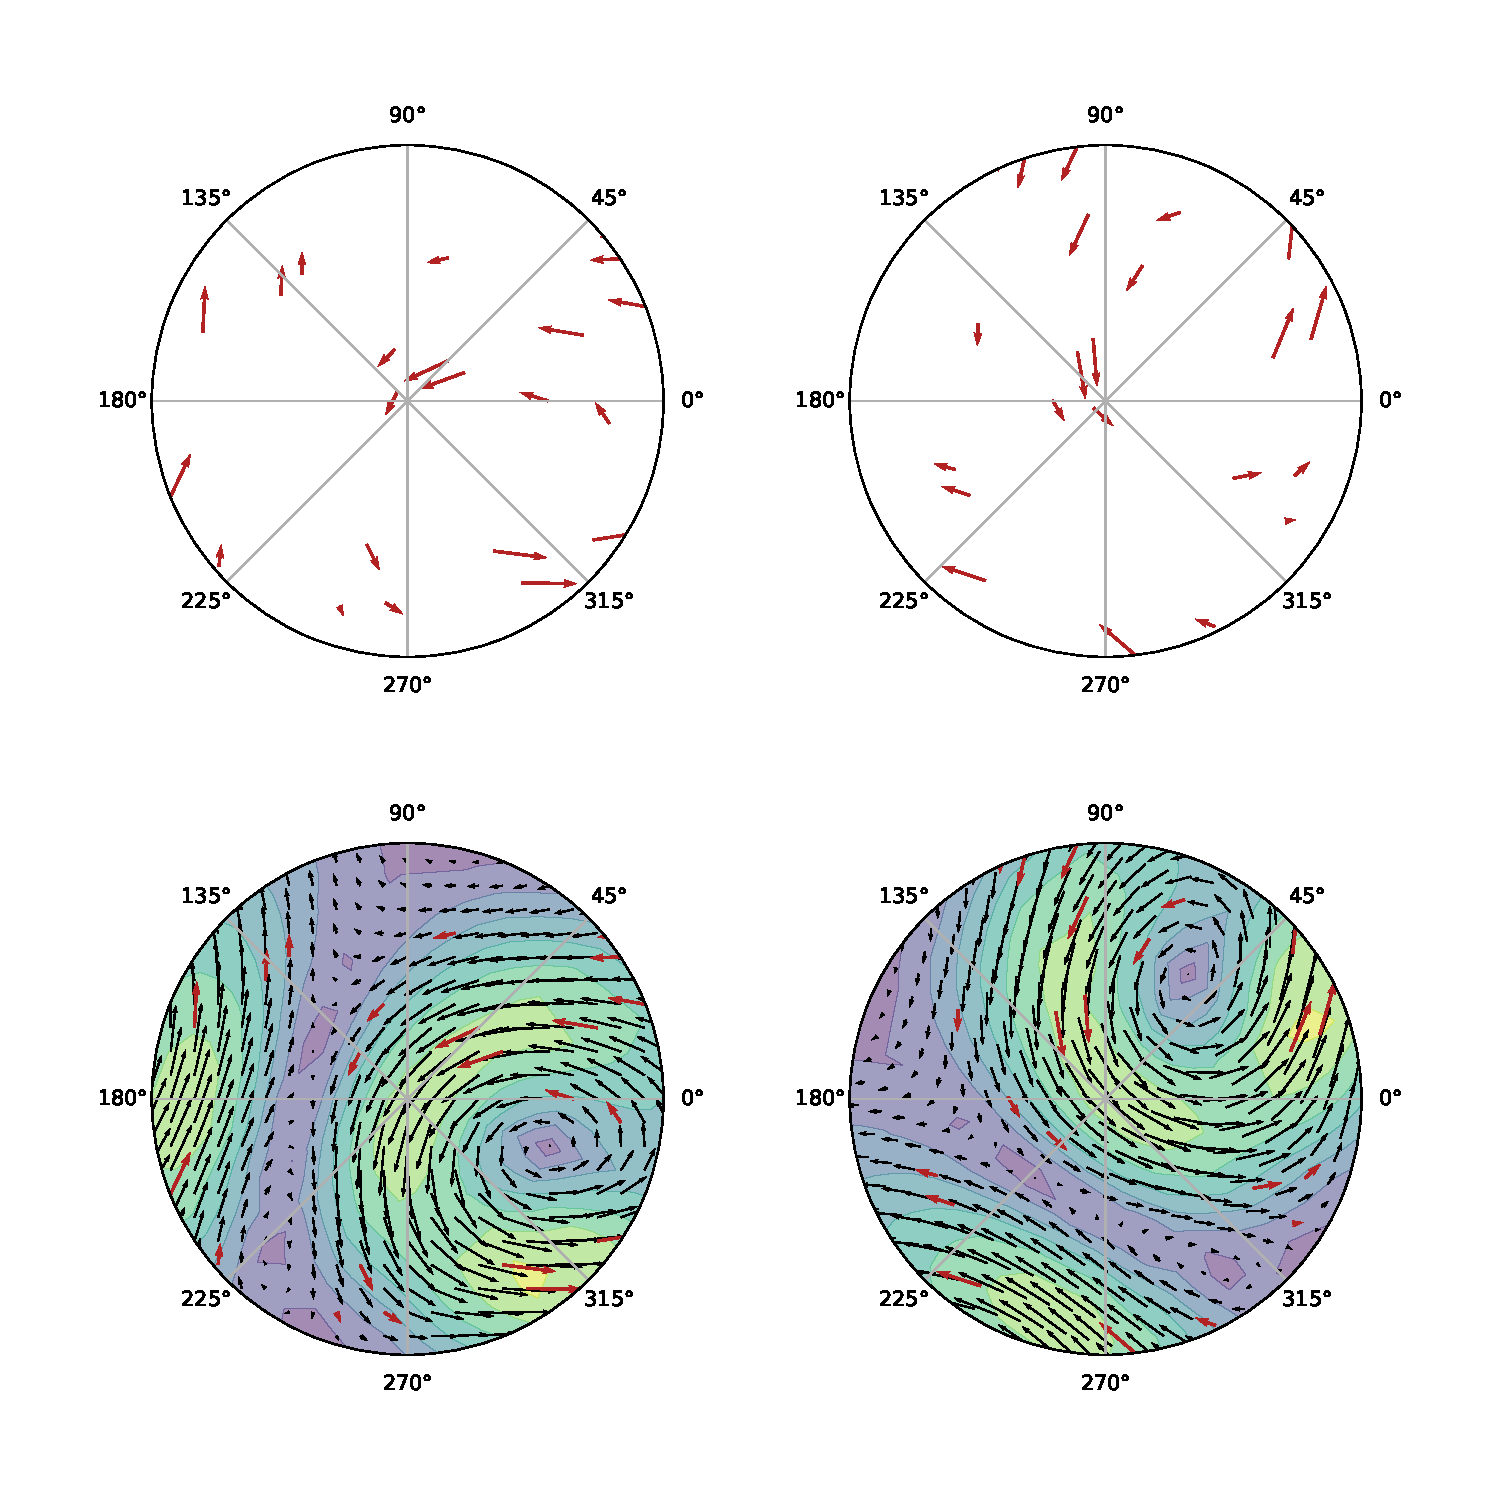
\includegraphics[width=0.9\textwidth]{Equiv_illustration.pdf}};
	\begin{scope}[x={(image.south east)},y={(image.north west)}]
	    \node (A) at (0.1, 0.4) {};
	    \node (B) at (0.1, 0.6) {};
	    \node (C) at (0.4, 0.1) {};
	    \node (D) at (0.6, 0.1) {};
 	    \node (E) at (0.9, 0.4) {};
 	    \node (F) at (0.9, 0.6) {};
 	    \node (G) at (0.4, 0.9) {};
 	    \node (H) at (0.6, 0.9) {};
        %\draw[red,ultra thick,rounded corners] (0.62,0.65) arrow (0.78,0.75);
        \draw[arrow] (B) -- node[anchor=west] {prediction} (A);
        \draw[arrow] (C) -- node[anchor=south] {rotation} (D);
        \draw[arrow] (F) -- node[anchor=east] {prediction} (E);
        \draw[arrow] (G) -- node[anchor=north] {rotation} (H);
    \end{scope}
\end{tikzpicture}

\end{document}